\chapter{楕円幾何学（リーマン幾何学）}

鈍角仮説においては、直線は有限の長さを持ち、自身へと戻る閉じた線となる。任意の2直線は合同変換によって重ね合わせることができるため、すべての直線はまったく同一の有限の長さを持つ。2直線は常に必ず交わり、同一の直線に対して垂直な2本の直線は、その直線から測って「直線の全長の半分」の距離にある点において互いに交差する。

\begin{figure}[htbp]
\centering
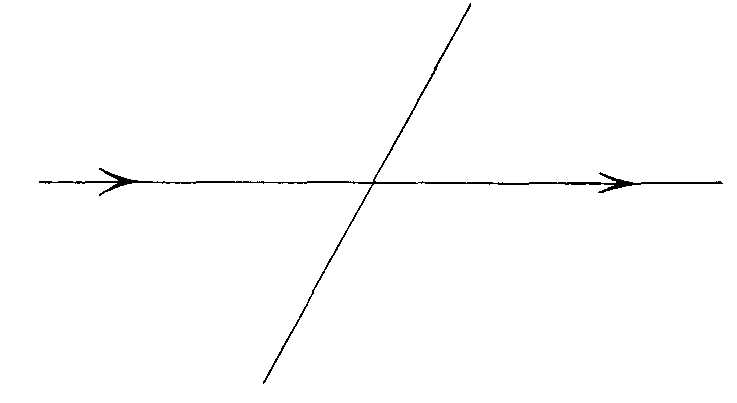
\includegraphics[width=70mm]{fig58.png}
\caption{楕円平面における直線と極・極線の構造}
\end{figure}

\begin{enumerate}[label=\textbf{\arabic*.}]
\item \textbf{直線は平面を2つに分割しない}：
2直線の交点を出発し、一方の直線に沿ってある有限の距離を進むと、他方の直線を一度も横切ることなく再び元の交点へと戻ってくることができる。すなわち、直線を横断することなく、その直線の「一方の側」から「他方の側」へと移動することが可能である（メビウスの帯・射影平面のトポロジー）。

与えられた直線に対するすべての垂線はある1点で交わる。この点をその直線の\textbf{極（pole）}と呼び、直線はその極の\textbf{極線（polar）}と呼ばれる。極から極線までの距離は「直線の全長の半分」であり、極線は極からこの等距離にある点の軌跡である。したがって、ある直線の極が別の直線の上にあれば、第2の直線の極は第1の直線の上にあり、2直線の交点は、両者の極を結ぶ直線の極となる。

与えられた直線から一定の距離にある点の軌跡は、その直線の極を中心とする円となる。直線とは、半径が直線の全長の半分に達したときの円の極限形式に他ならない。

互いに直交する3本の直線を描くことができ、これによって\textbf{3直角三角形（三直角三角形）}が形成される。この三角形は\textbf{自己極三角形（self-polar triangle）}でもあり、各頂点は対辺の極となっている。

\item \textbf{空間における極と平面}：
空間内において、ある平面に対するすべての法線は1点で交わり、この点がその平面の\textbf{極}となる。極は、半径が直線の全長の半分に達したときに平面を極限形として含む球面系の中心である。

平面上の図形は、平面の極を中心とする任意の球面上にある相似な図形から射影することができる。すなわち、対応する角は等しく、対応する辺の長さは球の半径のみに依存する一定の比率を持つ。

したがって、楕円平面上の幾何学は球面幾何学に酷似しているが、楕円平面は球面全体の「半分」（対蹠点を同一視した半球）に対応する。球面の中心を通る直径が球面の半分の点に対応するのと同様である。半球の境界にある直径の両端点が互いに同一である（貼り合わされている）と想像すれば、その半球は楕円平面と厳密に対応する。楕円平面には境界となる特定の直線は存在せず、すべての直線は対等である。平面は有界（限界）を持たないが、有限の広がり（面積）しか持たない。

直線の全長を $\pi$ とするような長さの単位系を選ぶと、球面三角法の公式が一切の変更なしにそのまま楕円平面に適用できる。直線上の距離は、その直線が極において張る中心角と同一の尺度を持ち、2直線のなす角はそれらの極の間の距離に等しくなる。任意の点からその極線までの距離（直線の全長の半分）は、これを\textbf{象限（quadrant, $\pi/2$）}と呼ぶことができる。

互いに直交する3つの平面と、それらの交点を極とする平面をとることにより、\textbf{自己極四面体}を作ることができる。この四面体の各頂点は対面の極であり、各頂点には3直角の三面角が存在し、各面は3直角三角形である。
\end{enumerate}

\begin{tcolorbox}[colback=white,colframe=blue!75!black,title=\textbf{定理 3}]
\emph{一定の直線に垂直なすべての平面は、別の固定された直線において交わる。この直線をもとの直線の\textbf{極線（共役線：conjugate）}と呼ぶ。この関係は相互的（相反的）であり、一方の直線上のすべての点は、他方の直線上のすべての点からちょうど象限（$\pi/2$）の距離にある。}
\end{tcolorbox}

\begin{figure}[htbp]
\centering
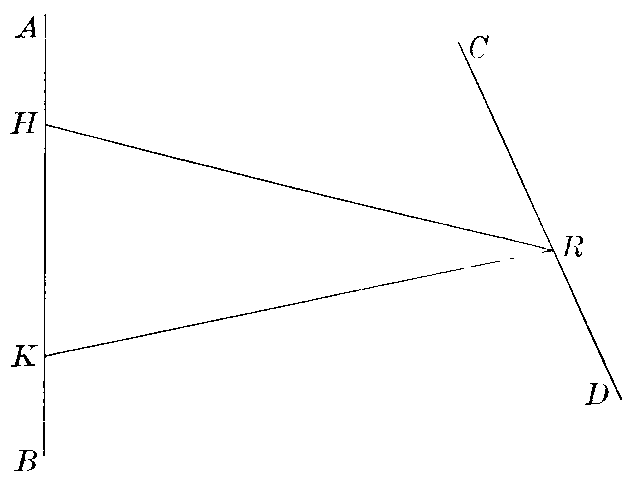
\includegraphics[width=60mm]{fig59.png}
\caption{共役直線と極線の相互関係}
\end{figure}

\textbf{【証明】}
直線 $AB$ に点 $H, K$ で垂直な2つの平面が直線 $CD$ で交わるとする。$AB$ および $CD$ 上の任意の点 $R$ を通る平面を考える。この平面は与えられた2つの平面とそれぞれ $HR$ および $KR$ で交わる。$HR, KR$ はともに $AB$ に垂直であるから、点 $R$ は点 $H, K$ の双方から象限の距離にある。したがって $R$ は、線分 $AR$ と点 $R$ で定まる平面において $AB$ の極であり、$AB$ 上のすべての点から象限の距離にある。
しかし $R$ は $CD$ 上の任意の点であったから、いずれの直線上の任意の点も、他方の直線上の各点から象限の距離にある。自己極四面体の対向する辺は互いに極線（共役線）の関係にある。

与えられた直線と直角に交わるすべての直線は、その共役線とも直角に交わる。したがって、任意の点から2つの共役線への距離は同一の直線上で測られ、その和は常に1象限（$\pi/2$）に等しい。ある直線から等距離にある2点は、その共役線からも等距離にある。

固定された直線から一定の距離にある点の軌跡は、その直線とその共役線の双方を回転軸とする回転面となる。これを\textbf{二重回転面（surface of double revolution）}と呼ぶ。一方の軸に関する緯線円は、他方の軸に関する子午線曲線となる。空間全体がある直線に沿ってその周りの回転を伴わずに移動するとき、空間はその共役線を軸として滑りを伴わずに回転する。直線に沿った平行移動と直線の周りの回転を組み合わせた運動を\textbf{ねじれ運動（screw motion）}と呼ぶ。したがって、ねじれ運動は2つの共役線のそれぞれに関する回転、または2つの共役線のそれぞれに沿った平行移動として記述できる。

\begin{tcolorbox}[colback=white,colframe=blue!75!black,title=\textbf{定理 4（クリフォードの平行線）}]
\emph{楕円幾何学においては、同一平面上にない直線でありながら、無数の共通垂線を持ち、至る所等距離であるような直線の対が存在する。}
\end{tcolorbox}

\begin{figure}[htbp]
\centering
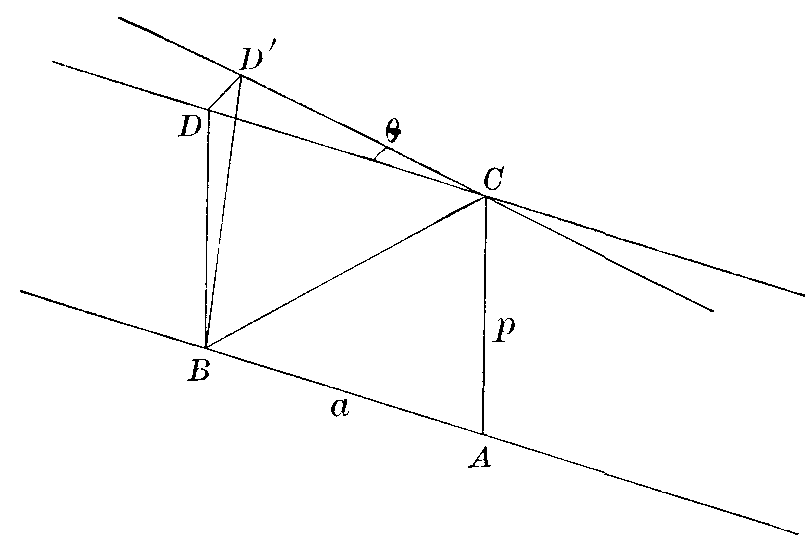
\includegraphics[width=80mm]{fig60.png}
\caption{クリフォードの平行線（至る所等距離な非共面直線）}
\end{figure}

\textbf{【証明】}
同一平面上にある任意の2直線とその共通垂線 $AC$ を考える。この垂線からいずれかの方向に進むと、2直線は互いに接近する。いま、一方の直線を共通垂線 $AC$ の周りに回転させ、2直線がもはや同一平面上にないようにする。ある特定の角度だけ回転させたとき、これら2直線は無数の共通垂線を持ち、その全長にわたって至る所等距離となる。

共通垂線 $AC$ の長さを $p$ とし、2直線上で垂線の足から同じ側に距離 $a$ にある点 $B, D$ をとる。同一平面上にあるときは $BD < p$ であるが、$CD$ を $AC$ の周りに $90^\circ$ 回転させると、$BD$ は $p$ より大きくなる。なぜなら $\triangle BCD$ は直角三角形となり、斜辺が $BD$、一辺が $BC$（直角三角形 $\triangle ABC$ の斜辺）となるため、$BD > BC > AC = p$ となるからである。

したがって、$CD$ がある角度 $\theta$ だけ回転したとき、$BD$ はちょうど $p$ に等しくなり、位置 $BD'$ をとる。三角形 $\triangle ABC$ と $\triangle D'BC$ は3辺がそれぞれ等しいため合同である。ゆえに $BD'$ は $CD'$ に垂直である。同様に $BD'$ は $BA$ にも垂直である。したがって、$BD'$ は $CA$ と同様に、直線 $AB$ と $CD'$ の双方に対する共通垂線となる。

点 $C$ において、3つの稜 $CB, CD, CD'$ を持つ三面角を考える。稜 $CD$ に沿った二面角は直角であるから、球面直角三角形の基本公式より以下が成り立つ：
\[
\cos \angle BCD' = \cos \angle BCD \cos \angle DCD'
\]
ここで $\angle BCD = \frac{\pi}{2} - \angle ACB, \quad \angle BCD' = \angle ABC$ であるから、
\[
\cos \angle ABC = \sin \angle ACB \cos \theta
\]
一方、直角三角形 $\triangle ABC$ において $\sin \angle ACB = \frac{\cos \angle ABC}{\cos p}$ が成り立つから、これを代入すると、
\[
\cos \theta = \cos p \implies \theta = p
\]
が得られる。驚くべきことに、この回転角 $\theta$ は距離 $a$ に一切依存しない。
したがって、平面上の任意の2直線に対し、一方をその共通垂線の周りに「その垂線の長さに等しい角 $\theta = p$」だけ回転させれば、得られる2直線は至る所完全に等距離となる。\hfill$\blacksquare$

\bigskip
楕円幾何学には通常の意味での平行線（交わらない同一平面上の直線）は存在しないため、このような至る所等距離な直線の対に対して\textbf{「平行線（クリフォードの平行線）」}という名称が与えられている。

空間の任意の点を通って、与えられた直線に対して2本のクリフォード平行線を引くことができる。これらは\textbf{右巻き（right-wound）}および\textbf{左巻き（left-wound）}として区別される。これらはすべて、与えられた直線を軸とする二重回転面上に完全に横たわっている。したがって、この二重回転面は一葉双曲面のように2組の直線母線を持つ\textbf{直紋面（ruled surface）}であり、その上には完全なユークリッド幾何学が実現されている（クリフォード・トーラス）。
